\section{Klassen, Features und Selektoren}
    \label{section:conceptClassesFeaturesSelectors}
    Das \gls{wccs} führt eine Klassifizierung der Inhalte von Webseiten durch.
    Dieses Kapitel erläutert, was eine Klasse im Kontext des \glspl{wccs} ist
    und mit welchen anderen Konzepten es in Beziehung steht.

    \subsection{Klassen}
        Der Begriff "`Klasse"' stammt aus der Mathematik und beschreibt eine Menge von Objekten,
        die eine gemeinsame Aussage erfüllen \cite{oberschelp:Mengenlehre}.
        Eine Klasse kann deshalb eindeutig gebildet werden.
        Diese Definition erfährt für das \gls{wccs} eine Erweiterung,
        die in Abbildung \ref{image:conceptClasses} modelliert wird.

        \begin{figure}[htb]
            \centering
            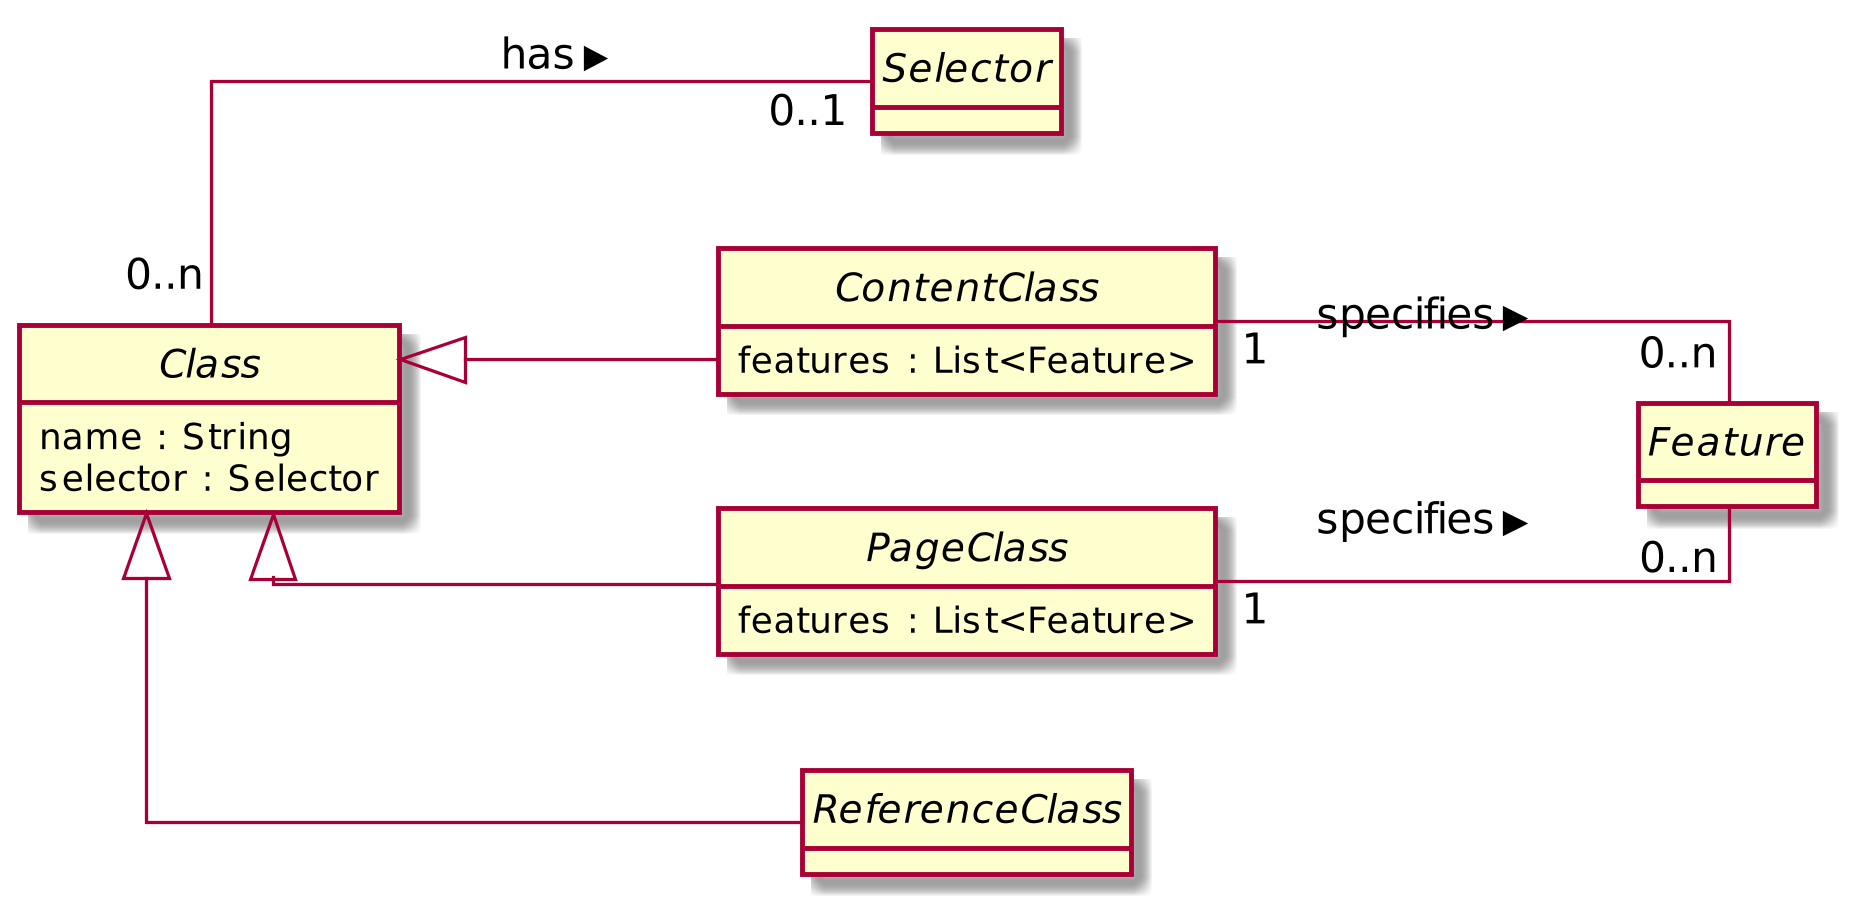
\includegraphics[scale=\imageScalingFactor]{../resources/concept/classes.png}
            \caption{Klassen im Kontext des WCCS'}
            \label{image:conceptClasses}
        \end{figure}

        Die zu klassifizierenden Entitäten sind Seiten, Inhalte und
        Referenzen\footnote{vgl. Kapitel \ref{section:classificationEntities}},
        weshalb das System drei Arten von Klassen kennt:

        \begin{enumerate}
            \item Seitenklassen,
            \item Inhaltsklassen und
            \item Referenzklassen.
        \end{enumerate}

        Allen Klassen ist gemein, dass sie einen Namen und bis zu einem Selektor haben,
        der darüber entscheidet, ob ein präsentiertes Objekt der Klasse zugehörig ist.
        Weshalb dieser Selektor optional ist, wird in Kapitel \ref{section:conteptSelectors} beschrieben.
        Seiten- und Inhaltsklassen besitzen Features,
        die zur Modellierung der komplexen Strukturen von Webseiten und ihren Inhalten dienen.
        Das \gls{wccs} sieht nicht vor, dass Referenzen solche Strukturen besitzen,
        weshalb Referenzklassen keine Features definieren.
        Jedes Feature ist in konkreten Klassifikationen als optional anzusehen,
        damit kleine Unterschiede in sonst sehr ähnlichen Webseiten keine neuen Klassen erforderlich machen.

    \subsection{Features}
        \label{section:conceptFeatures}
        Eine Webseite besitzt eine hierarchische inhaltliche Struktur,
        die durch ihre Klassifikation abgebildet werden muss\footnote{vgl. Kapitel \ref{section:requirements}}.      
        Dazu führt das \gls{wccs} das Konzept der Features ein,
        die Teil einer Seiten- oder Inhaltsklasse sind.
        Ein Feature besitzt selbst ebenfalls eine Klasse,
        welche ihrerseits wiederum Features enthalten kann.
        Die Klassendefinitionen erhalten dadurch eine beliebig komplexe hierarchische Struktur,
        um den erwarteten Aufbau eines klassifizierten Objektes zu modellieren.
        Innerhalb einer Klassifikation stehen Features also in einer Teil-Ganzes-Beziehung zu einander.
        Um Bezug auf ein übergeordnetes Feature zu nehmen,
        wird im weiteren Verlauf dieser Arbeit der Ausdruck "`\parentFeature"' verwendet.
        Ein untergeordnetes Feature wird entsprechend "`\childFeature"' bezeichnet.
        Abbildung \ref{image:conceptFeatures} zeigt eine ausführlichere
        konzeptionelle Darstellung von Features im \gls{wccs}.

        \begin{figure}[htb]
            \centering
            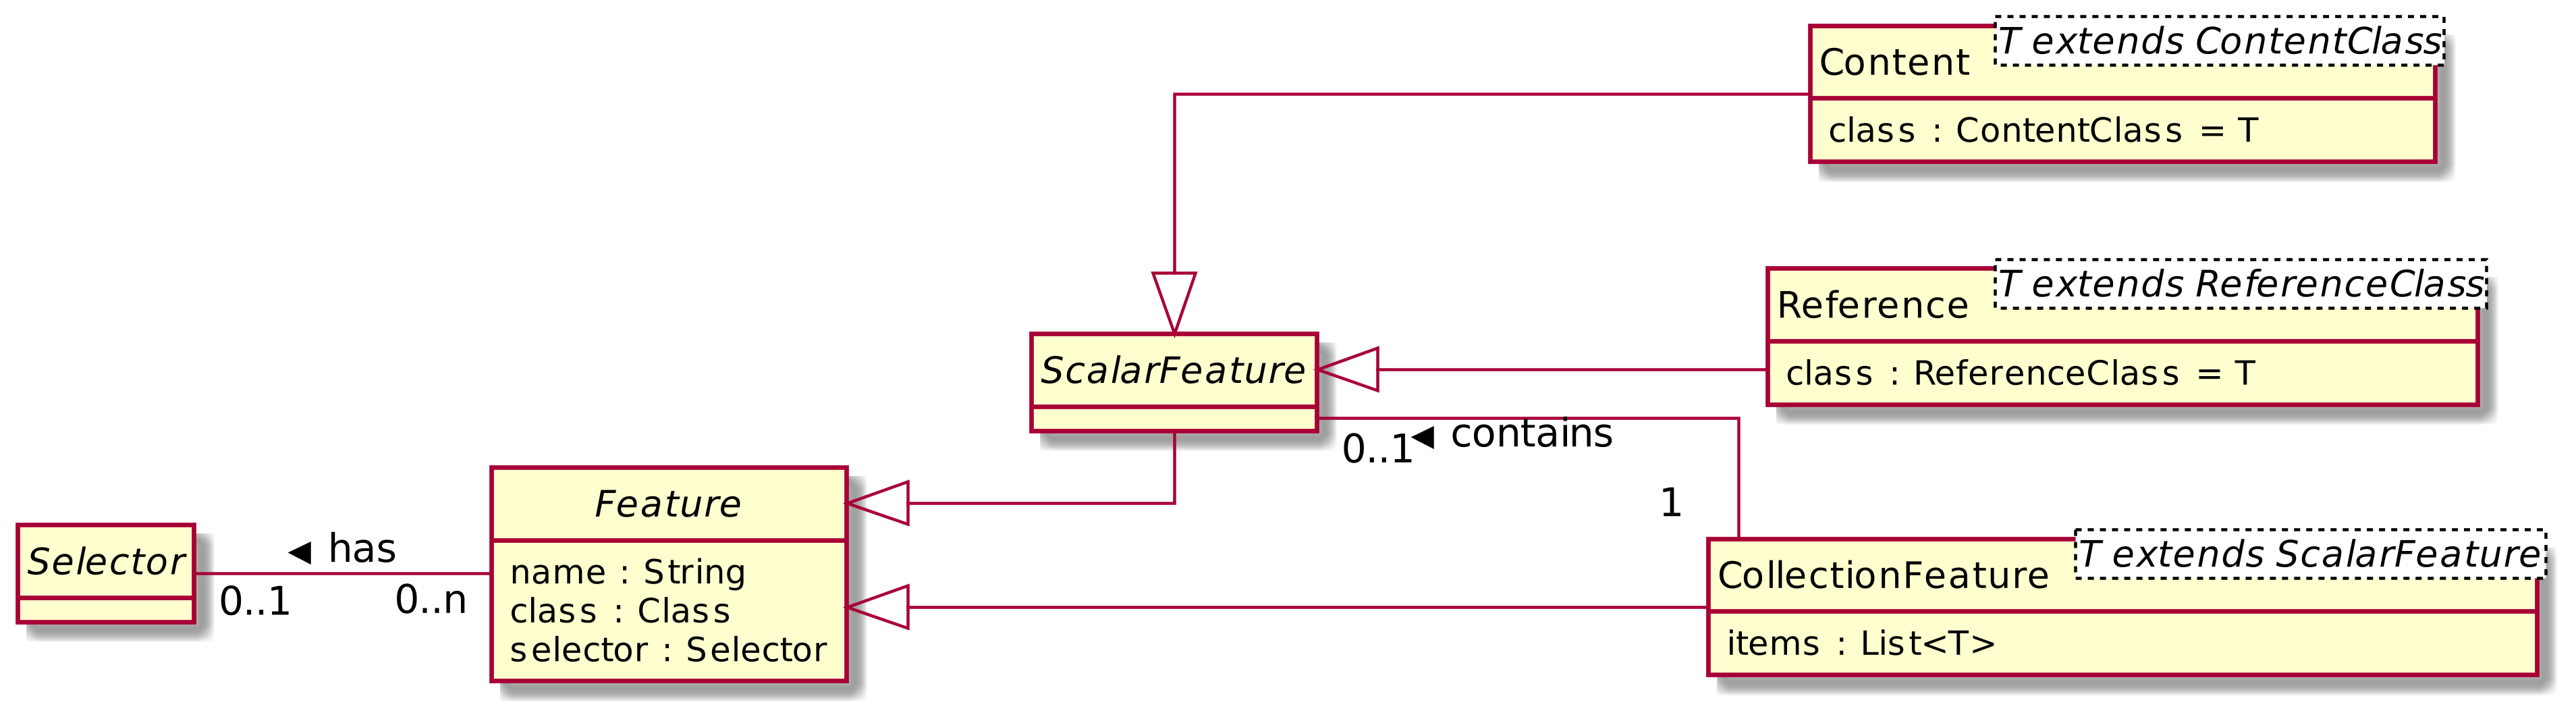
\includegraphics[scale=\imageScalingFactor]{../resources/concept/features.png}
            \caption{Features im Kontext des WCCS'}
            \label{image:conceptFeatures}
        \end{figure}

        Das \gls{wccs} unterscheidet zwei konkrete Arten von Features:
        
        \begin{enumerate}
            \item Inhalt, die im weiteren Verlauf auch als {\contentFeature}s bezeichnet werden, und
            \item Referenzen, die auch {\referenceFeature}s genannt werden.
        \end{enumerate}

        {\contentFeature}s klassifizieren textuelle Inhalte,
        weshalb die Klasse solcher Features auch eine Inhaltsklasse sein muss.
        Entsprechend muss die Klasse einer Referenz eine Referenzklasse sein.
        Jedes Feature besitzt neben einer Klasse auch einen Namen und wie Klassen optional einen Selektor.
        Die Frage, warum sowohl Klassen als auch Features Selektoren besitzen,
        beantwortet Kapitel \ref{section:conteptSelectors}.

        Neben der Art des klassifizierten Objektes unterscheidet das \gls{wccs} Features
        außerdem anhand ihrer Kardinalität.
        Einelementige Features, sogenannte {\scalarFeature}s, enthalten die Klassifikation genau eines Objektes.
        {\collectionFeature}s hingegen speichern eine Menge von Klassifikationen,
        um sich wiederholende Elemente unter einem Namen zusammenzufassen.
        Jede einzelne Klassifikation in dieser Menge ist wiederum ein {\scalarFeature},
        von denen jedes diesselbe Klasse besitzen muss.
        In Abbildung \ref{image:conceptFeatures} wird dies durch die Typerweiterung an
        \texttt{CollectionFeature}, \texttt{Content} und \texttt{Reference} angezeigt.
        Prinzipiell könnte man {\scalarFeature}s auch durch einelementige {\collectionFeature}s realisieren,
        allerdings bringt die Unterscheidung auch eine Semantik mit sich und drückt eine
        Erwartungshaltung bezüglich klassifizierter Objekte aus.       
        Einelementige {\collectionFeature}s oder viele Treffer für ein {\scalarFeature}
        können zum Beispiel auf inkorrekte Selektoren oder nicht beachtete Unterschiede zwischen Webseiten hindeuten.

    \subsection{Selektoren}
        \label{section:conteptSelectors}
        Die bisher beschriebenen Konzepte dienen der Spezifikation von komplex strukturierten Klassen.
        Um eine Klassifizierung durchzuführen, benötigt das \gls{wccs} aber auch Merkmale,
        anhand derer es entscheiden kann,
        welche Elemente einer Webseite es welchen Klassen zuweist.
        Diese Merkmale werden mithilfe von Selektoren ausgedrückt,
        für die es abstrakt gesehen zwei Anwendungsfälle gibt:

        \begin{enumerate}
            \item Eine gegebene Webseite als Ganzes einer Seitenklasse zuweisen und
            \item Features innerhalb eines bereits klassifizierten Elementes ausfindig machen.
        \end{enumerate}

        Um den ersten Fall möglich zu machen,
        muss jede Definition einer Seitenklasse auch die Angabe eines Selektors enthalten,
        sodass eine konkrete Webseite gegen jede Seitenklasse geprüft werden kann.
        Features benötigten zur Laufzeit ebenfalls einen Selektor,
        allerdings kann dieser unterschiedlich ermittelt werden.
        Die erste Möglichkeit ist den Selektor der Inhalts- oder
        Referenzklasse des Features zu verwenden.
        Es erscheint allerdings sinnvoll, diesen Standardwert bei Bedarf für einzelne Features
        zu überschreiben, um Unregelmäßigkeiten einzelner Webseiten zu kompensieren.
        Der Selektor kann deshalb auch Teil eines Features sein.
        Die Spezifikation eines Selektors ist aus diesem Grund sowohl
        bei Klassen als auch bei Features optional,
        da nur sichergestellt sein muss, dass zum Zeitpunkt der Klassifizierung für jedes
        Feature ein Selektor ermittelt werden kann.        
        Es wird nicht ausgeschlossen, dass der gleiche Selektor von mehreren Klassen verwendet wird,
        was die Möglichkeit eröffnet, konkrete Inhalte und Referenzen mehreren Klassen zuzuweisen.

        Das \gls{wccs} unterstützt verschiedene Arten von
        Selektoren\footnote{vgl. Kapitel \ref{section:conceptClassification}},
        um ein breites Spektrum an Möglichkeiten anzubieten.
